%% sigconf for double column
%% natbib for bibtex
%% nonacm because it is not for a conference
\documentclass[format=sigconf, natbib=true, nonacm=true]{acmart}
\usepackage{lipsum}
\usepackage{hyperref}
\begin{document}
    \title{Impact on End-users by ISP IPv6 Deployment}

    \author{Tim Niklas Gruel}
    \affiliation{
    \institution{Ruhr-Universität Bochum}
    \city{Bochum}
    \country{Germany}
    }
    \email{tim.gruel@rub.de}

    \begin{abstract}
        This paper presents an overview about different techniques to cope with the IPv4 address exhaustion. The impact on the end-users is on focus. First some early NAT based solutions are introduced. Later dualstack is discussed. At the end the IPv6 only solution, deployed by ISPs today, is presented. It turns out that the end-user, especially the technical experienced one, can experience great benefits with IPv6. With IPv6 the internet gets back to its routs. All devices can talk to each other and central server are not mandatory to establish communication.
    \end{abstract}

    \keywords{IPv6, Tunneling, Translation, End-user Impact, NAT64, DNS64, 464XLAT, Dualstack}

    %% page numbers
    \settopmatter{printfolios=true}

    \maketitle

    \section{INTRODUCTION}
    In the late 90s is became very clear, that the IPv4 address space is not sufficient to meet the future demand. The popularity of the Internet especially in the end-user marked was heavily underestimated at the creation of IPv4. There are approximately 4 billion IPv4 addresses. Today there are over 8 billion humans on earth. That means that two humans need to share a single IPv4 address, not considering servers. Today, a typical family has multiple devices per person, including TVs, gaming consoles, smart phones, personal computers and many more. This led to the assignment of the last available IPv4 block in the early 2010s. With the rise of smart home technology and IoT devices, the demand for IP addresses per houshould will not stop to incrise.In this paper I will present a nearly complete overview over the different idears to slow down the inevitable IPv4 exhaustion. Expect for the last one, none of these is a long term solution or even tries to solve the problem itself. ISPs tried to keep cost as low as possible. This led to keeping IPv4 addresses as long as possible.\\\\First, ISPs started to assign only one public IP per customer. The customer had to use NAT44 in order to provide all his end devices with an internet connection. The end-user was the one getting a worse experience. Over the time, assigning only one IPv4 per customer was too much for the ISPs. Especially with the rise of mobile internet and an even higher demand for addresses, IPv4 was doomed. ISPs tried to provide more IP addresses, by only assigning private IPv4s to customers, leading to NAT444. NAT itself has many problems, which will be discussed in this paper. NAT444 makes the problems even worse. End-users were and are still heavily effected by that.\\\\A few years later dualstack was provided by the ISPs. Dualstack introduced the next generation of IP addresses, called IPv6. Compared to IPv4 addresses which are a 32 Bit string, IPv6 addresses are a 128 Bit string. IPv6 solves the problem of address exhaustion completly. Unfortunately IPv6 is not backwards compatible to IPv4. Thus all infrastructure needs to be renewed. The Internet is fully decentralices. It is not possible to perform such a transition on one particular day. Dualstack implements both, IPv4 and IPv6. Devices and servers supporting IPv6 can communicate over IPv6. In the case that one device is not yet capable of IPv6, IPv4 acts as a fallback. This is a perfect transition technology, but it is no solution for the IPv4 exhaustion problem. Each end-user still needs an public or private IPv4. The problem is not solved.\\\\Lately, ISP started to provide IPv6 only. This is also very common in mobile networks. The devices natively speak to servers over IPv6. For legacy IPv4 servers, there are different translation mechanisms. This paper will look deeper into NAT64 combined with DNS64. Moreover I will present 464XLAT. Both are similar to a NAT44, but tranlating between IPv6 and IPv4. The interesting thing is, that these translation happens at the ISP, so the end-user only works with IPv6. This has many advantages for the end-user. Though, some legacy applications depending heavily on IPv4 cannot be used. One example for that is Skype.\\\\At the end of this paper, tunneling IPv6 in IPv4 and the other way around is presented. This happens only at ISP level, but indirectly influences the end-user to. Mainly in a better path availability, thus seemless internet service. There are many technologies, including 6in4, 6to4, 6over4, 6rd, Teredo, 4in6.\\\\In the last few years the apodption of IPv6 has increased rapidly. On \url{https://www.google.com/intl/en/ipv6/statistics.html} it is possible to view the current adoption of IPv6 regarding the Google landing page. Germany for example has an adoption of over 65\%. This statistics really shows the trend of ISPs worldwide, deploying IPv6 only or dualstack. Nearly all mobile clients use IPv6 today and are able to interact with the Internet without major notable disadvantages. Cisco predicts that the transition to IPv6 is finished in 2028. This means that nerly all end-users and servers world wide communicate over IPv6. That has great advantages for the end-user regarding security and opens up entirely new options for innovative peer to peer technologies. Hosting a Server on a smart phone might sound strange today, but could be a very usual thing in 10 years from now. The end-user is the one benefiting the most from unique, world-wide routable IP addresses.\\\\Now I am going to turn back the time a bit and we are focussing on the problem, emerging in the late 90s. It becomes clear that the IPv4 address space is not big enough. ISPs are searching for a solution. The main goal is to assign the same public, gloably routable IPv4 address to multiple devices. This is not meant for a long period of time, but much more as a quick fix, until the new standard IPv6 is developed.
    
    \section{EARLY SOLUTIONS}
    This section presents three different solution to to extend the lifetime of IPv4. I will discuss NAT44, A+P and NAT444. All these solutions aim to share one single IPv4 address between multiple end devices. It is important to understand theses technologies in order to correctly estimate the impact of IPv6 deployment by ISPs. Evaluating modern solutions alone could leed to the impression, that these solutions are better or worse than they really are. Thus this paper starts with NAT44.
    \subsection{NAT44}
    NAT44 is also kown as CPE NAT. The word NAT stands for \textit{Network Address Translation}. NAT44 means that one IPv4 address is translated to multiple IPv4 addresses. CPE means \textit{Customer Premises Equipment}. The whole NAT procedure is up to the end-user. The ISP only provides one single IPv4 address. Typically one public, globally routable IP is tranlated to multiple private IP addresses. There are three private IPv4 Blocks which are the following:
    \begin{enumerate}
        \item 10.0.0.0/8
        \item 172.16.0.0/12
        \item 192.168.0.0/16
    \end{enumerate}
    Everybody can use the IPv4 addresses in these blocks. Private IPv4 addresses will never be routed in the internet. Most end-users use the third option for their home network. Thus they can use 254 different devices which is sufficient for most users. All these 254 devices share one public IPv4. All of them share the $2^{16} = 65536$ ports of the public IPv4 too. From the outside you cannot decide whether only one device or multiple devices are behind the NAT.
    \begin{figure}
        \centering
        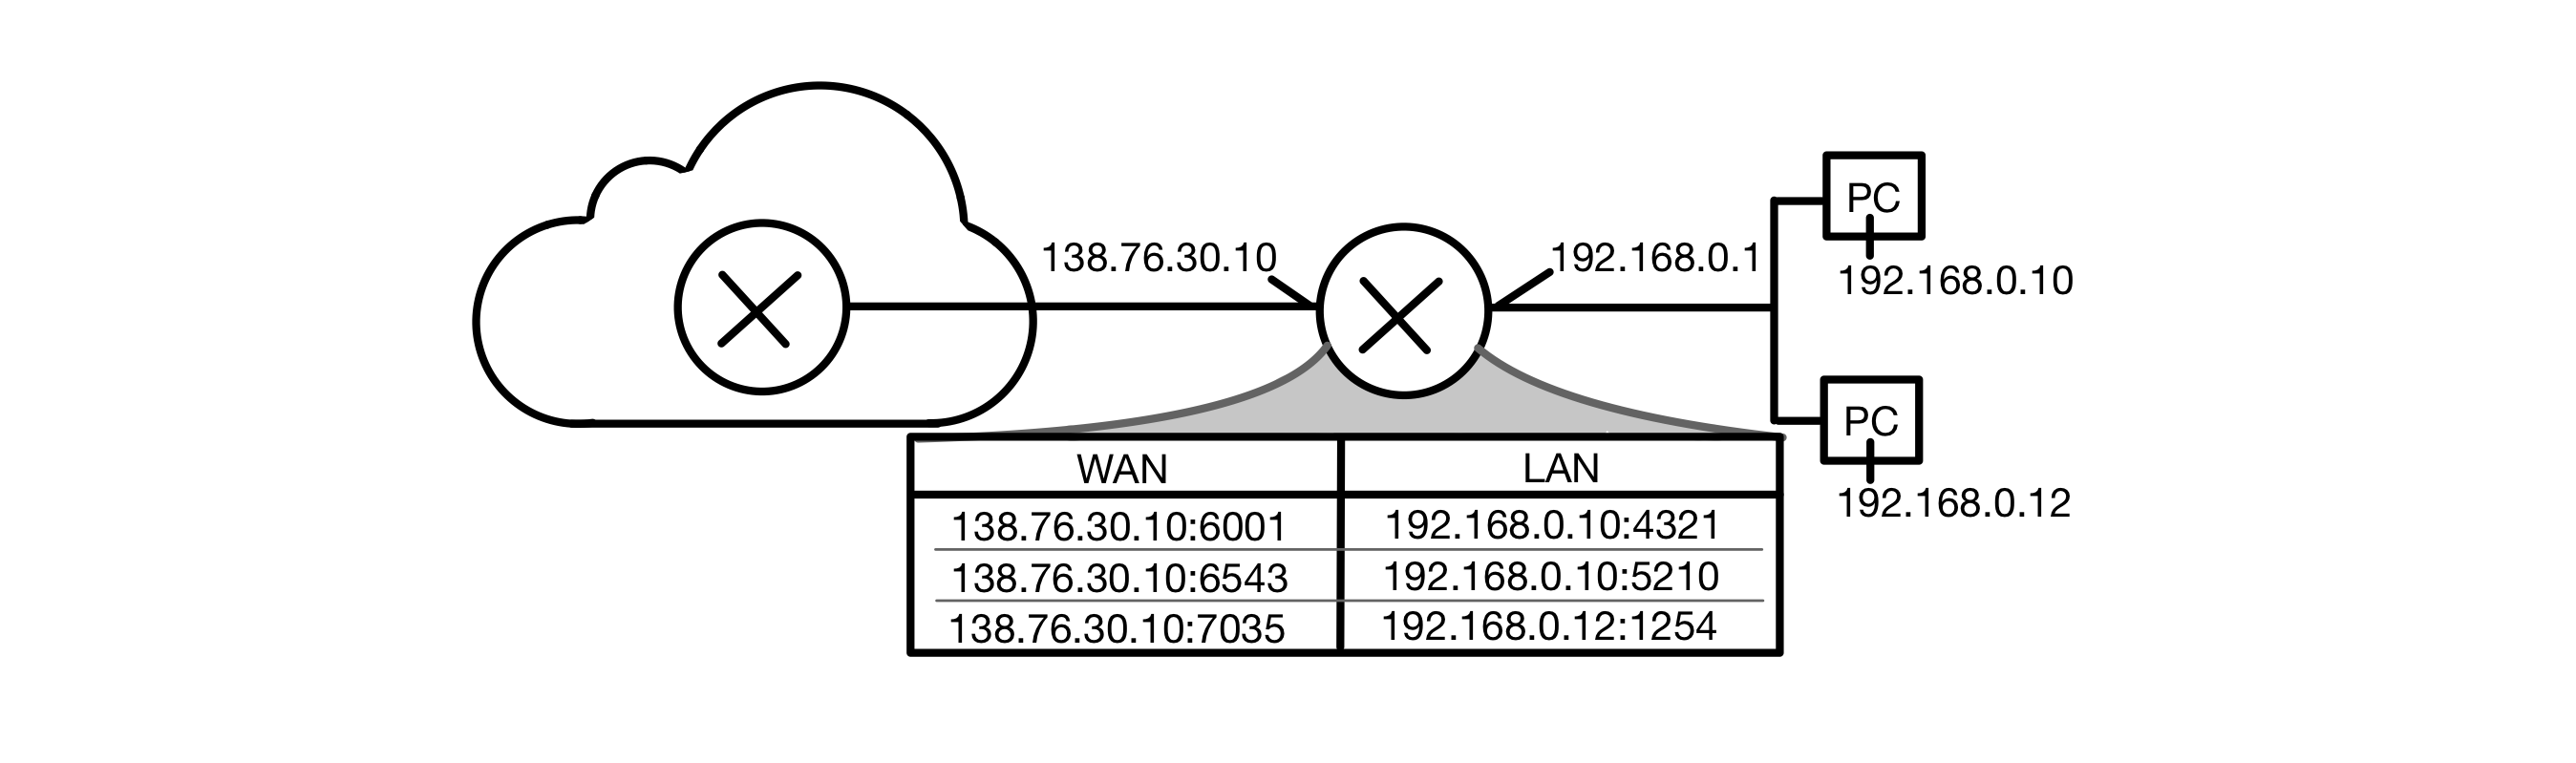
\includegraphics[width=0.5\textwidth]{images/nat_44.png}
        \caption{Example of NAT44 with NAT-Translation table}
        \label{fig:nat_44}
    \end{figure}
    In the example \ref{fig:nat_44} is a NAT-Translation table. As you can see, the PC with IP \textit{192.168.0.10} cannot use all ports, because the PC with the IP \textit{192.168.0.12} uses the Port \textit{7035}. All ports are shared. This can lead to problems as we discuss later. NAT44 was the first solution to the IPv4 exhaustion problem. It is an easy fix, because the ISP has nothing to change, except now only delivering one single IP per customer. The end-user needs a NAT compatible router.
    \subsection{A+P}
    A+P means \textit{Address Plus Port}. Over the time NAT44 was not a sufficient solution anymore. The demand for IPv4 rose and ISP were not able to provide one single public, globally routable IPv4 per customer. The idea is still very similar to NAT44, but with A+P each costumer gets one IPv4 and a designated port range. With that system it is possible to share one IP to theoretically \textit{65536} different customers \cite{8716482}.
    \begin{figure}
        \centering
        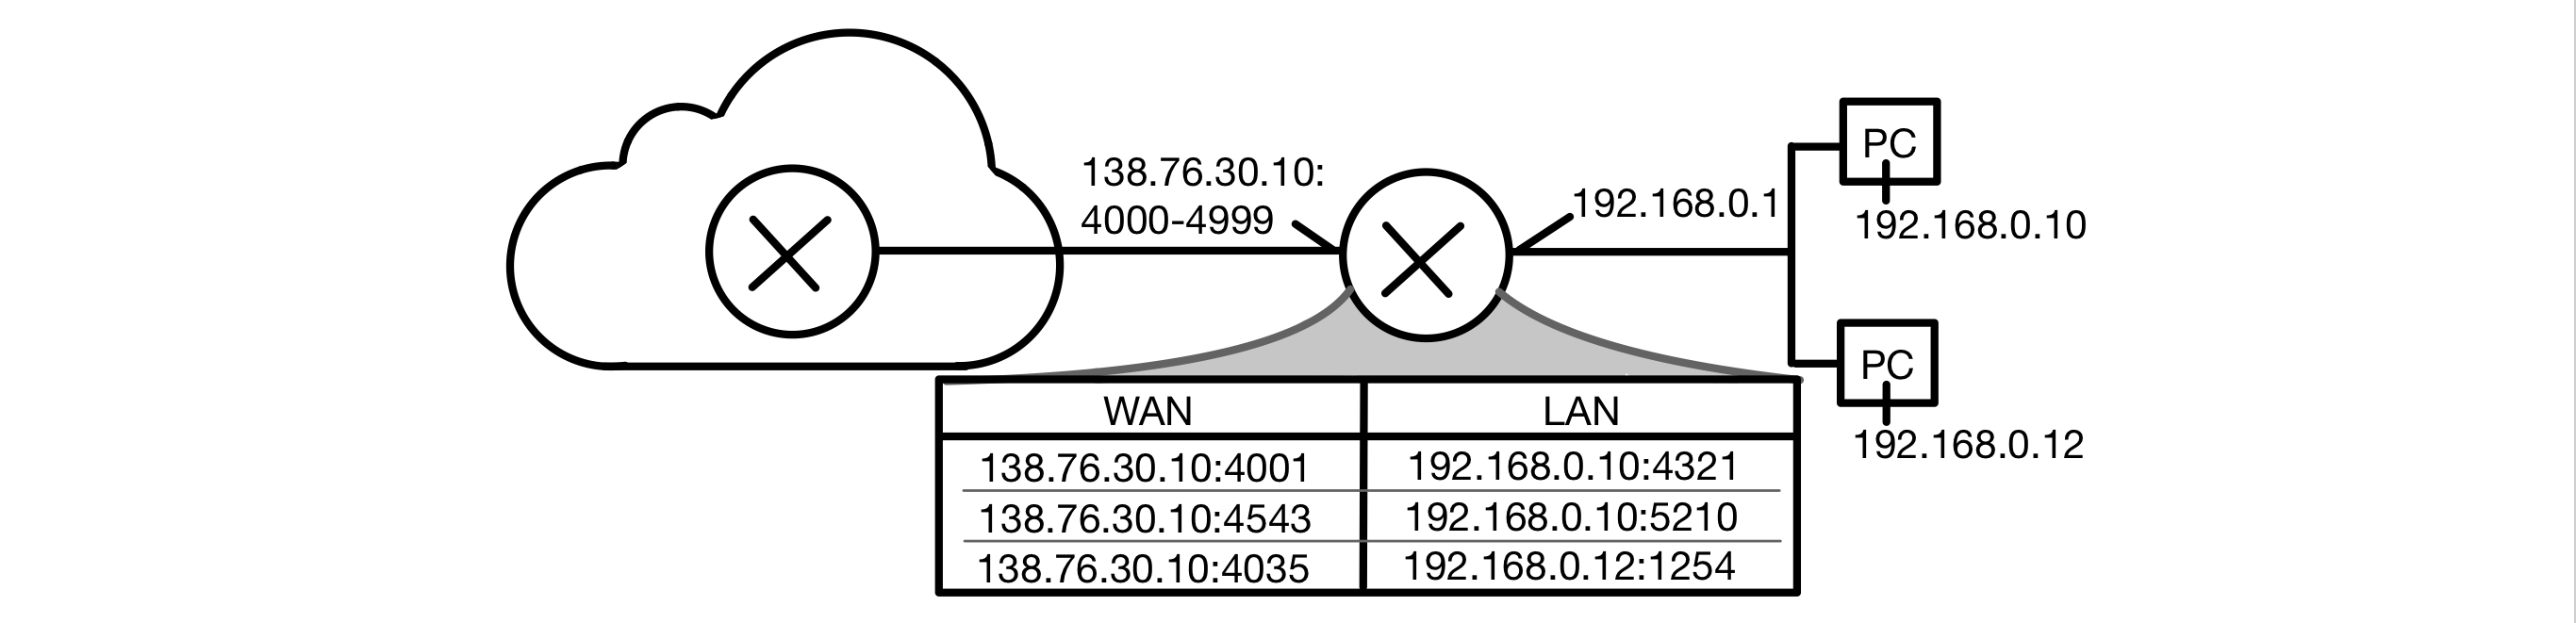
\includegraphics[width=0.5\textwidth]{images/a_plus_p.png}
        \caption{Example of A+P with NAT-Translation table}
        \label{fig:a_plus_p}
    \end{figure}
    In the example \ref{fig:a_plus_p} you can see that all internal ports are mapped to port values between \textit{4000} and \textit{4999}. This is because the ISP assigned this port range to that particular customer. All internal devices combined can open \textit{1000} ports. The biggest advantage of A+P is also the biggest downside. On the one hand, it is possible to supply more customers with public, globally routable IPv4 address, but on the other hand all these customers have a tiny available port range. Assuming the extreme case of \textit{65536} different customers, each customer would only get one single port. Even when ports are dynamically assigned, the user experience at peak internet usage time would be unacceptable.
    \subsection{NAT444}
    NAT444 is also knwon as CGN. CGN means \textit{Carrier Grade Natwork Address Translation}. With NAT44 one public, globally routable IPv4 address is translated to multiple private IPv4 addresses at ISP site. Each customer gets one private IPv4 address. Similar to NAT44, the customer than translates that private IPv4 into multiple private IPv4 address for all home devices. That means there is a double NAT. IP addresses get translated twice \cite{10.1145/2987443.2987474}. This leads to even more problems than NAT44 or A+P \cite{8716482}.
    \begin{figure}
        \centering
        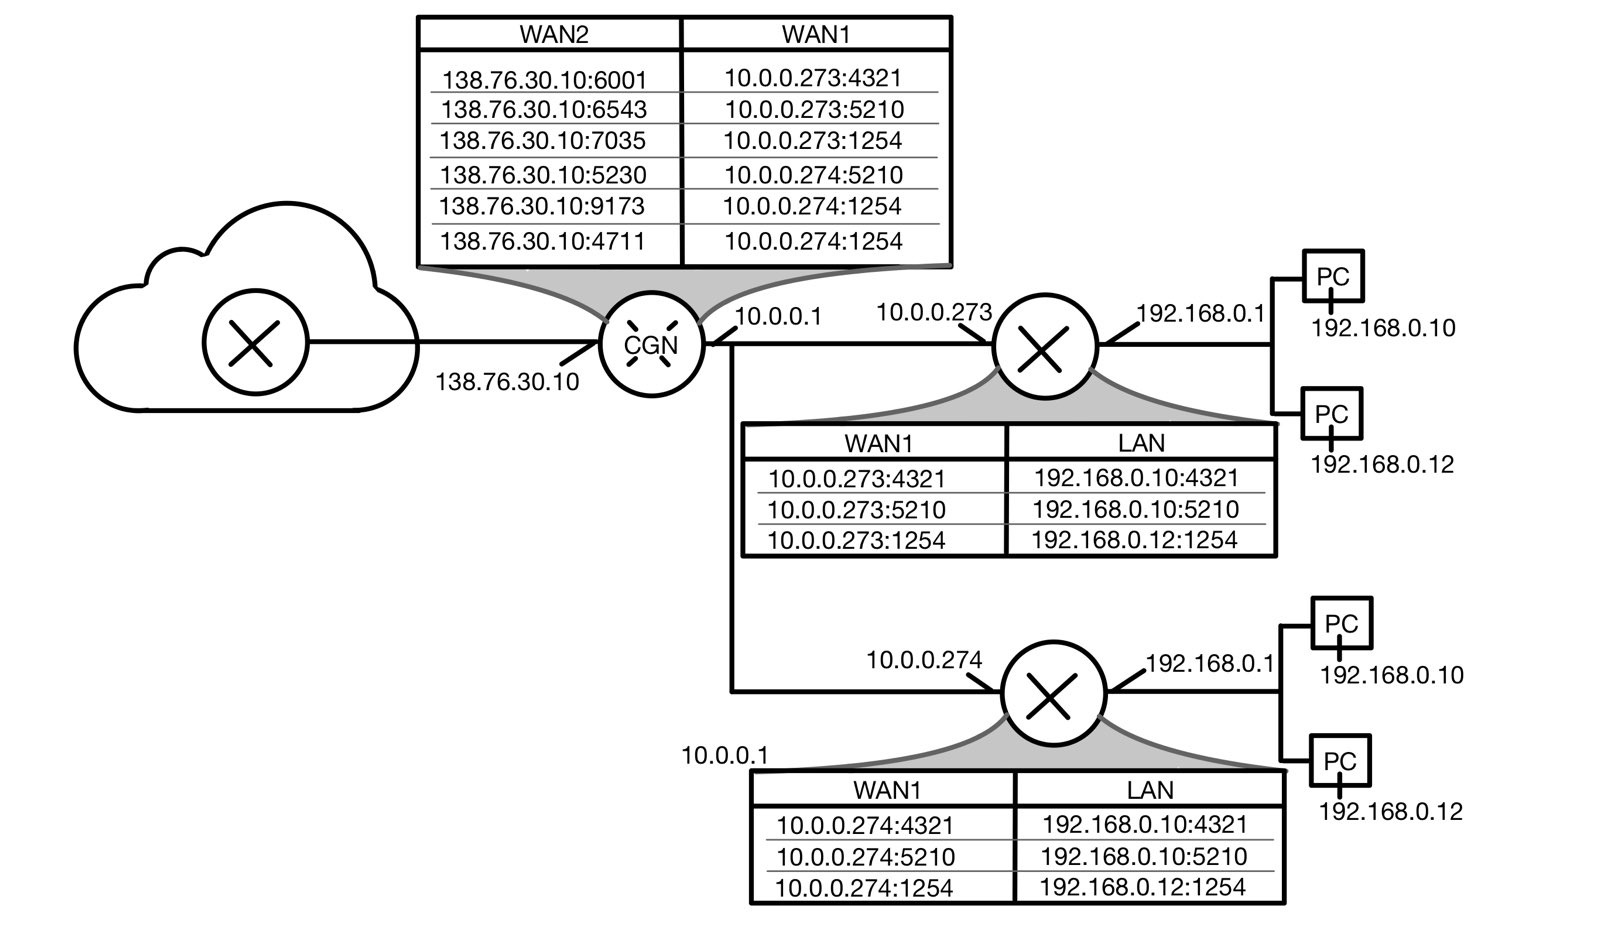
\includegraphics[width=0.5\textwidth]{images/nat_444.png}
        \caption{Example of NAT444 with translation tables}
        \label{fig:nat_444}
    \end{figure}
    In example \ref{fig:nat_444} two end-users are connected to the CGN. The CGN has the public, globally routable IPv4 \textit{138.76.30.10}. One customer gets assigned the private IPv4 \textit{10.0.0.273} and the other one the private IPv4 \textit{10.0.0.274}. Both operate a typical \textit{192.168.0.0/16} Network. As you can see, both customers have a personal computer with the private IPv4 \textit{192.168.0.10}. Yet the system works. After the end-user NAT translation, these personal computers have the IPv4 \textit{10.0.0.273} and \textit{10.0.0.274} with the corresponding ports. Then the CGN translates these private IPv4 addresses into the only public, globally routable IPv4 \textit{138.76.30.10}. The CGN translates IP and Port and maps them to the corresponding customer. In a real world application, the CGN would control multiple public, gloablly routable IPv4 addresses and split them between all customers. Example \ref{fig:nat_444} just shows a cutout of the whole CGN.
    \subsection*{END-USER IMPACT}
    NAT44, A+P and NAT444 cause very similar problems and have a huge impact on the end-user. Some of them will be discussed now.\\\\The first problem is regarding location services. Typically it is possible to determine a rough geolocation regarding one single public IPv4. Especially with NAT444 one IPv4 is shared by many users. Thus it is not really possible to accurately guess the location. Some people might argue that this is a advantage too, because it increases privacy\cite{Hughes2022_C04}.\\\\A very serious problem is regarding spam. IPv4 addresses distrubiting spam, typically can be blacklisted. With a shared IPv4 address between multiple end-users this can leed to blocking of innocent end-users who just were unlucky to share a IP with an adversary\cite{Hughes2022_C04}.\\\\Another problem is regarding peer-to-peer applications. To establish and mentain a peer-to-peer network it is necessary to ping a peer directly. This happens with a public IPv4 and a well kown port. With NAT that is generelly not possible. All devices share one IPv4 with all ports\cite{Hughes2022_C04}.\\\\Similar to peer-to-peer it is not possible to host own servers behind a NAT. Web servers for example establish \textit{https} connection over the well-known port \textit{443}. With NAT44 it is theoretically possible to forward a port to one device. Thus it is possible to operate one server of a kind per port. For example one web server and one ftp server. With A+P or NAT444 this option is completly gone and it is not possible to host servers. That impacts end-users massivly. The main idea of the internet is a decentraliced network. Everyone should be able to set up servers and start communications without a central instance. NAT disabled this main idea of the internet\cite{Hughes2022_C04}.\\\\Modern web applications nowadays usually require many ports to operate. With NAT these ports are limited and could run short. This is a very serious problem, because as it is not possible to create more IPv4 addresses, it is not possible to create more Ports\cite{Hughes2022_C04}.\\\\Apart from the obvious disadvantages, some protocolls like DNS are less secure with NAT. Because of the DNS poisoning attack, a client starts new DNS requests with a random port. Assuming that an attacker cannot guess the port, the DNS server answers to that port. If an attacker can guess the port and answer to it first, the attacker can infiltrate wrong DNS entries. This is a series security risk. With the use of NAT44 all devies share the available ports. The problem gets even worse with A+P or NAT444. If an attacker knows the assigned port range, the DNS cache poisoing attack is very effective. IPSec needed to be upgraded to work with NAT44 and currently does not work with NAT444\cite{Hughes2022_C04}.\\\\A generall problem with NAT is, that it is a single point of failure. If a personal NAT router or a CGN router is not working anymore, all clients cannot access the internet. A NAT router is a very lucrative attack target\cite{Hughes2022_C04}.\\\\In a nutshell, NAT has many problems. It was meant as a quick fix until the next generation of IP is finalized. Unfortunately, NAT outlived it supposed livetime by many years. This is why modern solutions are required to get away from NAT and return to the original open and accessable internet.
    \section{MODERN SOLUTIONS}
    It became very clear that IPv4 is not sufficient anymore. This is why IPv6 was standardized. IPv6 addresses are a \textit{128} bit string. With IPv6 it is possible to assign $2^{128}=3.4*10^{38}$ addresses. This number of addresses will suffice forever. IPv6 indefinitely solves the IPv4 exhaustion problem. Unfortunately IPv6 is not backwards compatible to IPv4. The first solution was to implement IPv6 alongside IPv4. This gives older applications the possibility to continue using IPv4 until they and the servers are upgraded. Assining both a IPv4 address and IPv6 addresses is called \textit{dualstack}. The two very similar technologies \textit{dualstack} and \textit{dualstack lite} are introduced now. They are meant to be transition technologies from the world of IPv4 only to IPv6 only.
    \subsection{DUALSTACK}
    With \textit{dualstack} the end-user gets a public, globally routable IPv4 address and a block IPv6 addresses from the ISP. With the IPv4 address, the end-user performs NAT44. This was discussed in the previous chapter. In addition to that private IPv4 address, all devices also get assigned a global, publicly routable IPv6 address \cite{8716482}. A personal computer now has two implemented IP layers as in \ref{fig:dualstack}. Old application that only support IPv4 work seamlessly without any modification required.
    \begin{figure}
        \centering
        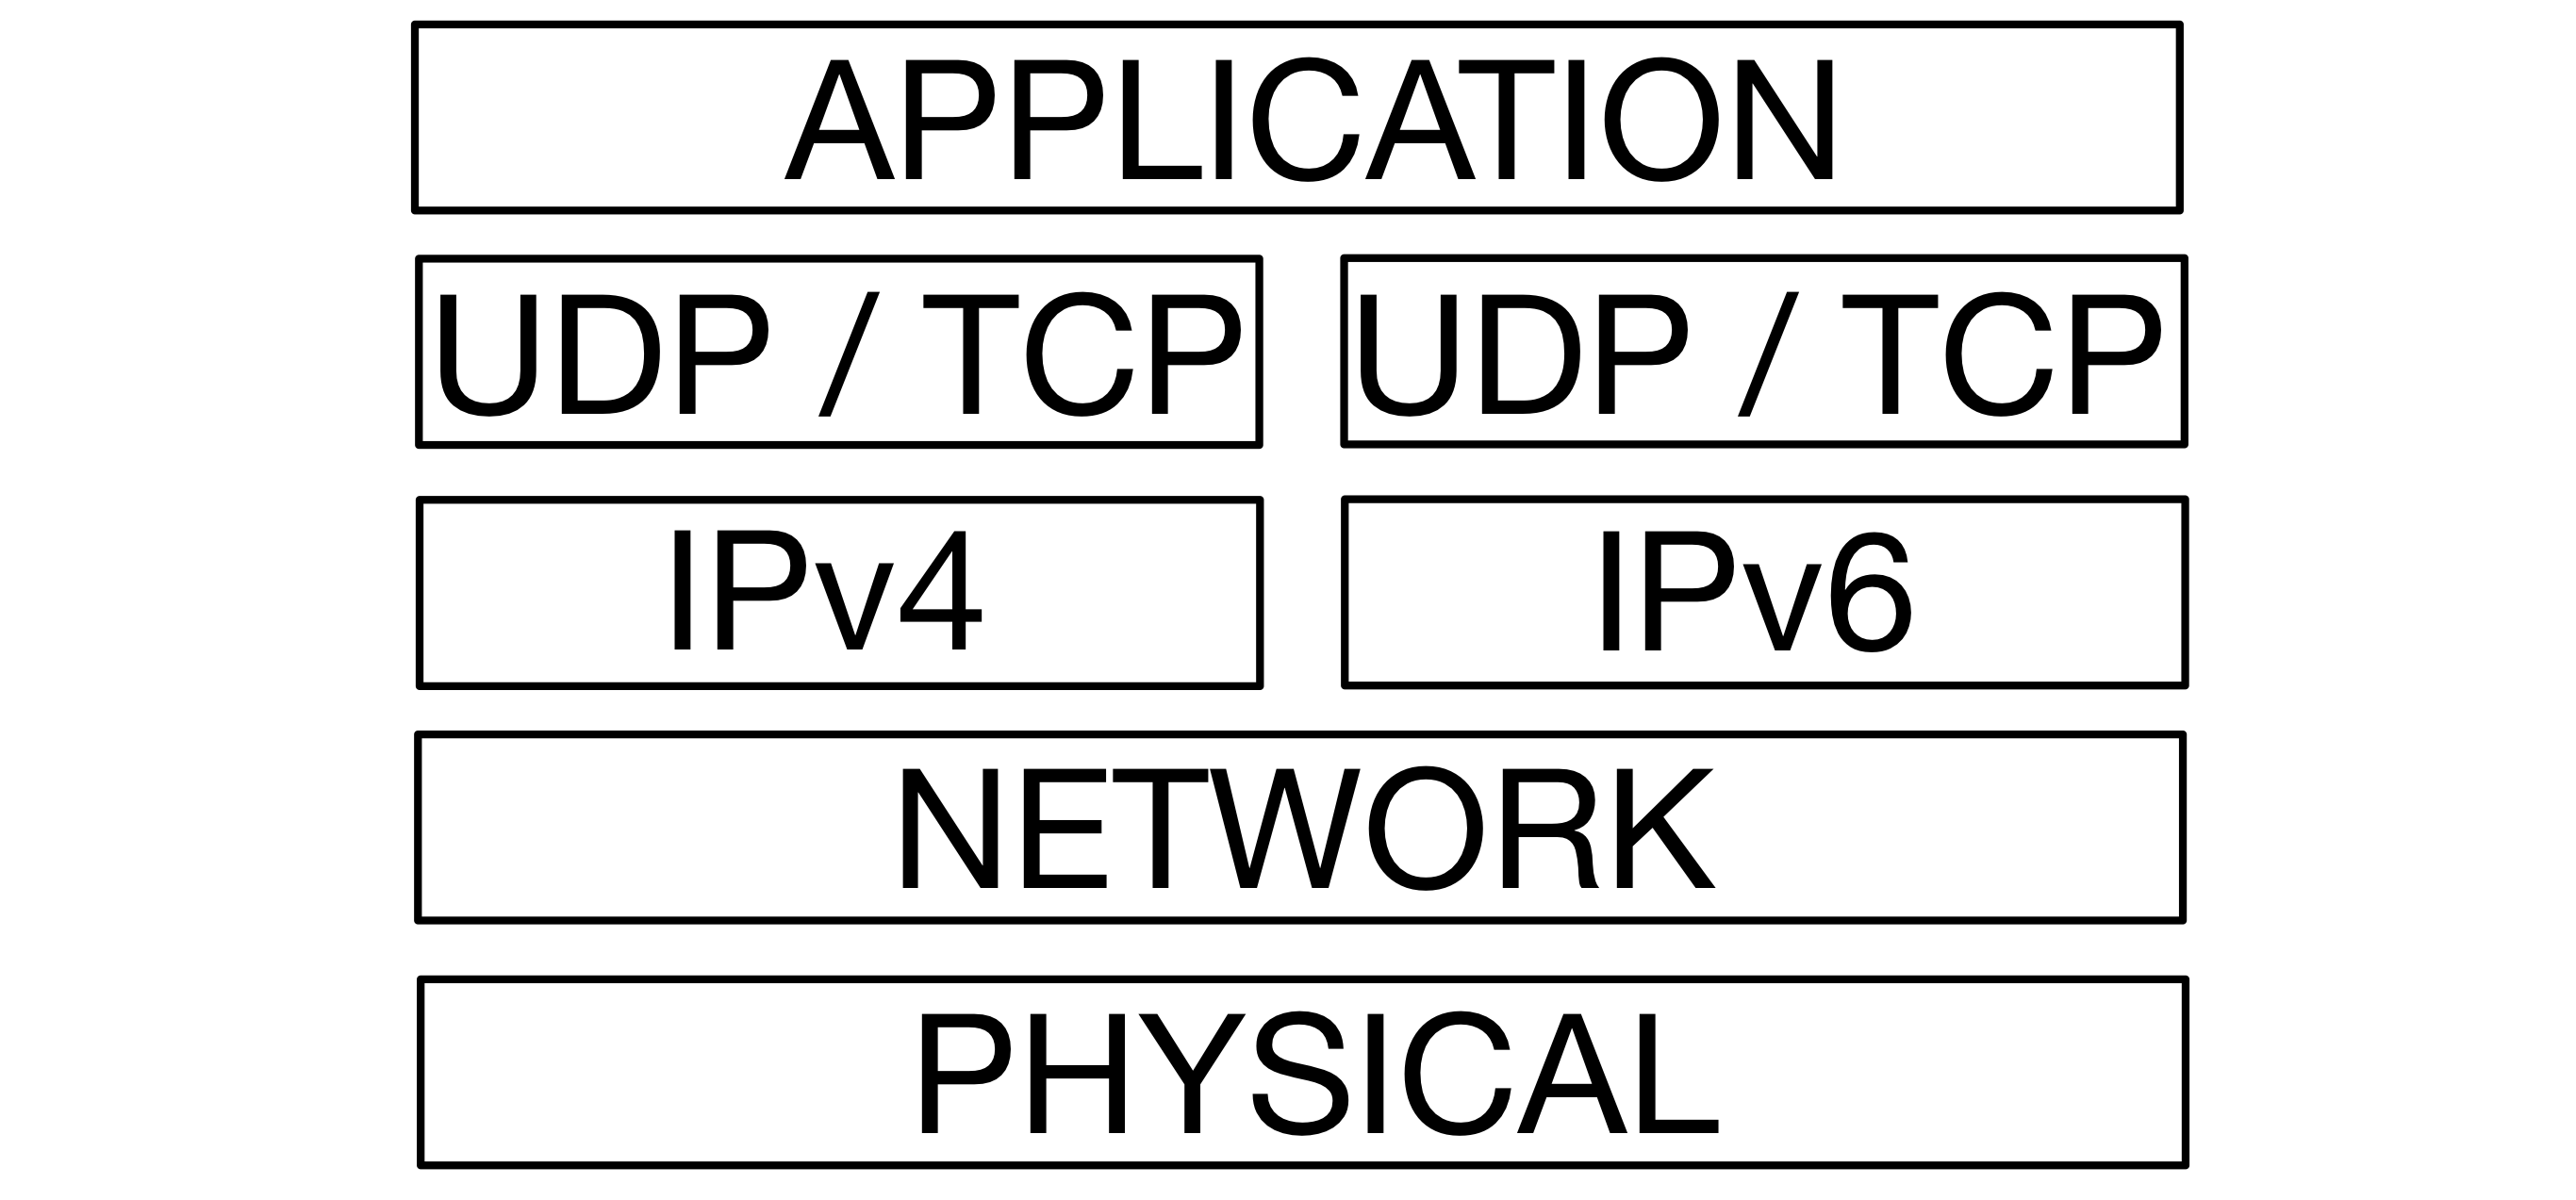
\includegraphics[width=0.5\textwidth]{images/dualstack.png}
        \caption{Dualstack IP layer implementation}
        \label{fig:dualstack}
    \end{figure}
    With IPv6 an ISP typically get a \textit{/32} network containing $2^{128-32}=2^{96}$ IPv6 addresses. The end-user then gets a \textit{/64} network. IPv6 addresses are noted as 8 two byte blocks divides by a colon. The example in \ref{fig:dualstack_network} shows a very basic end-user \textit{dualstack} network containing one router and two end-devices. The ISP got the \textit{2001:0db8:0000:0000:0000:0000:0000:0000/32} block assigned. The router implements NAT44 and got the block \textit{2001:0db8:0001:0002:0000:0000:0000:0000/64} assigned by the ISP. The router can now distribute the last 4 two byte blocks to the devices. In this example the two personal computers got the public, globally routable IPv6 \textit{2001:0db8:0001:0002:0000:0000:0000:0010} and \textit{2001:0db8:0001:0002:0000:0000:0000:0012}. In addition to that the router assigns the private IPv4 addresses \textit{192.168.0.10} and \textit{192.168.0.12} to the personal computers. An application on one personal computer can now use the private IPv4 address with all the disadvantages discussed earlier or use the IPv6 address.
    \begin{figure}
        \centering
        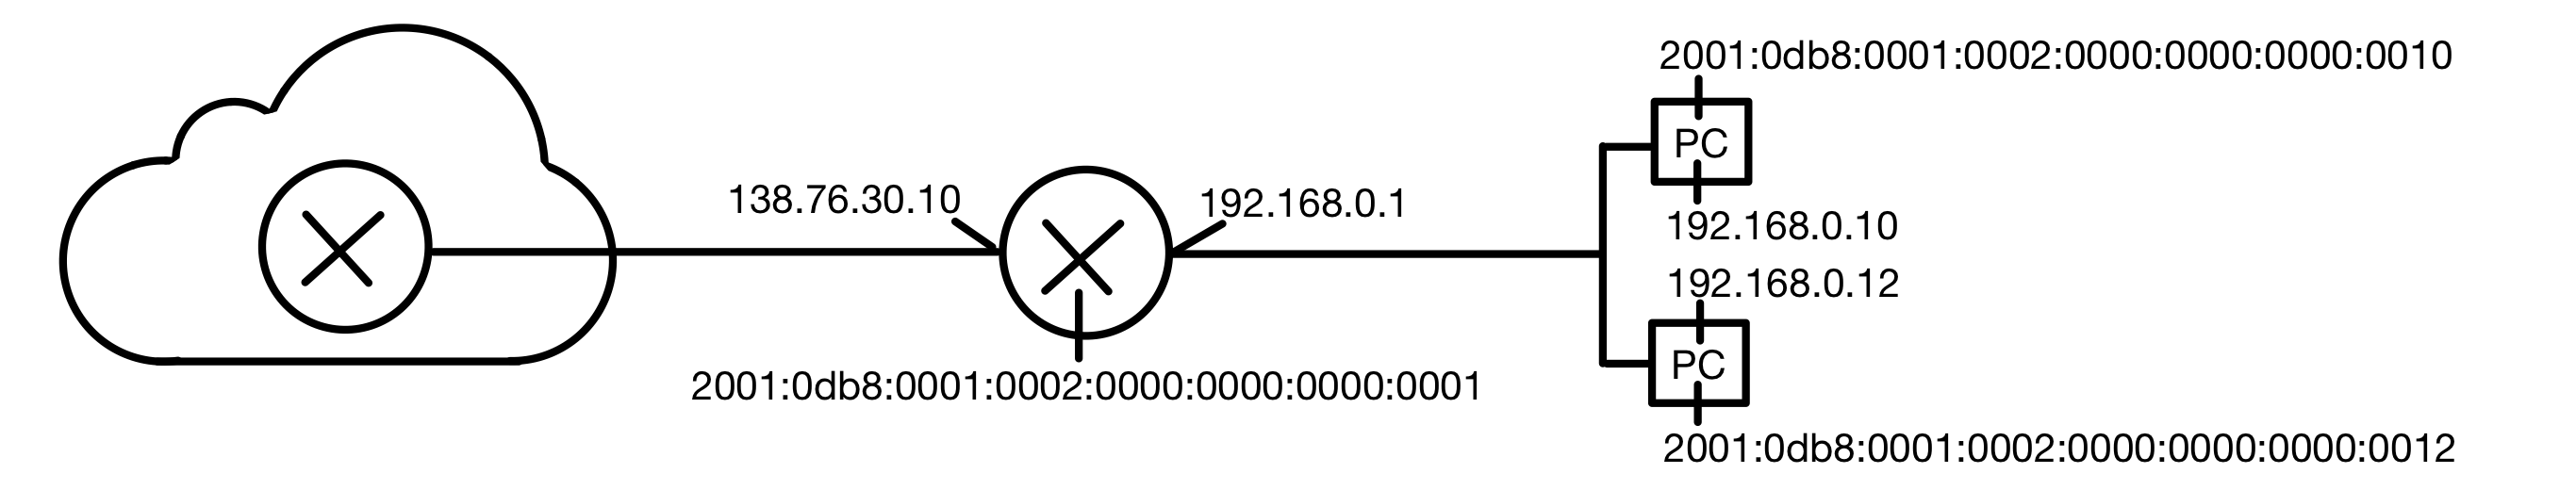
\includegraphics[width=0.5\textwidth]{images/dualstack_network.png}
        \caption{Example of a Dualstack network}
        \label{fig:dualstack_network}
    \end{figure}
    \subsection{DUALSTACK LITE}
    \textit{Dualstack Lite} also called \textit{DS Lite} is similar to \textit{dualstack} from a end-device point of view. An end-device gets a public, gloablly routable IPv6 address and a private IPv4 address. The end-device needs an \textit{dualstack} implementation as shown in \ref{fig:dualstack}. In case the device wants to communicate with an IPv4 legacy server, the device has to use the IPv4 stack and the private IPv4. In all other cases the public, gloablly routable IPv6 is preferred. There is no translation between IPv4 and IPv6 or the other way around. All in all \textit{dualstack} and \textit{dualstack lite} does not differ for the end-device.\\\\Compared to \textit{dualstack}, the network traffic between the router of the customer and the ISP is IPv6 only. IPv4 packets are tunneled in IPv6. The IPv4 packet is part of the data field of the IPv6 packet. DNS is done over IPv6 only. The \textit{B4} element will perform DNS for all clients in the network. Thus DNS is never routed to \textit{AFTR}.\\\\\ref{fig:dualstack_lite_network} is an example of a basic \textit{dualstack lite} setup. The customers router has a \textit{B4} element. This \textit{B4} element directly connects to the ISPs \textit{AFTR}. The \textit{B4} and \textit{AFTR} create an IPv6 tunnel for IPv4 packets. NAT44 is only applied at ISP level. Though, each customer hosts his own DHCPv4 Server to distribute IPv4 addresses in the home network. The IPv4 packets are packed into the IPv6 data field and directly send over IPv6 to the \textit{AFTR}. The \textit{AFTR} recieves the IPv6 packages and extracts the IPv4 packages. Now the AFTR does NAT44. In addition to the original private IPv4 address and the port, the NAT table also saves the assigned IPv6 block for the customer. Because of that, the end-user can theoretically use an arbitrary private IPv4 block\cite{rfc6333}. \ref{fig:dualstack_lite_network} shows that \textit{customer 1} and \textit{customer 2} both use the private IPv4 block \textit{192.168.0.0/16}. There are even two personal computer with both the private IPv4 \textit{192.168.0.12} in combination with the port \textit{3872}. This is no problem, because the NAT table also stores the customer assined IPv6 block. \textit{Dualstack Lite} allows nearly endless scaling. It is not necessary to assign one public IPv4 per costumer. Over the time, the workload for the NAT table will decline becuase more and more clients will use the superior public, globally routable IPv6 address. There are only two option, when IPv4 is needed. Either an legacy IPv4 application or device on the client side, or a device that wants to reach a server that is only capable of IPv4.\\\\\textit{Dualstack lite} also works with IPv4 only or IPv6 only devices. These only get assigned the corresponding IP address and work as intendet. \textit{Dualstack lite} only uses NAT44 similar to \textit{Dualstack}. That is why both are superior to \textit{NAT444}, while providing a usable solution even with IPv4 exhaustion.
    \begin{figure}
        \centering
        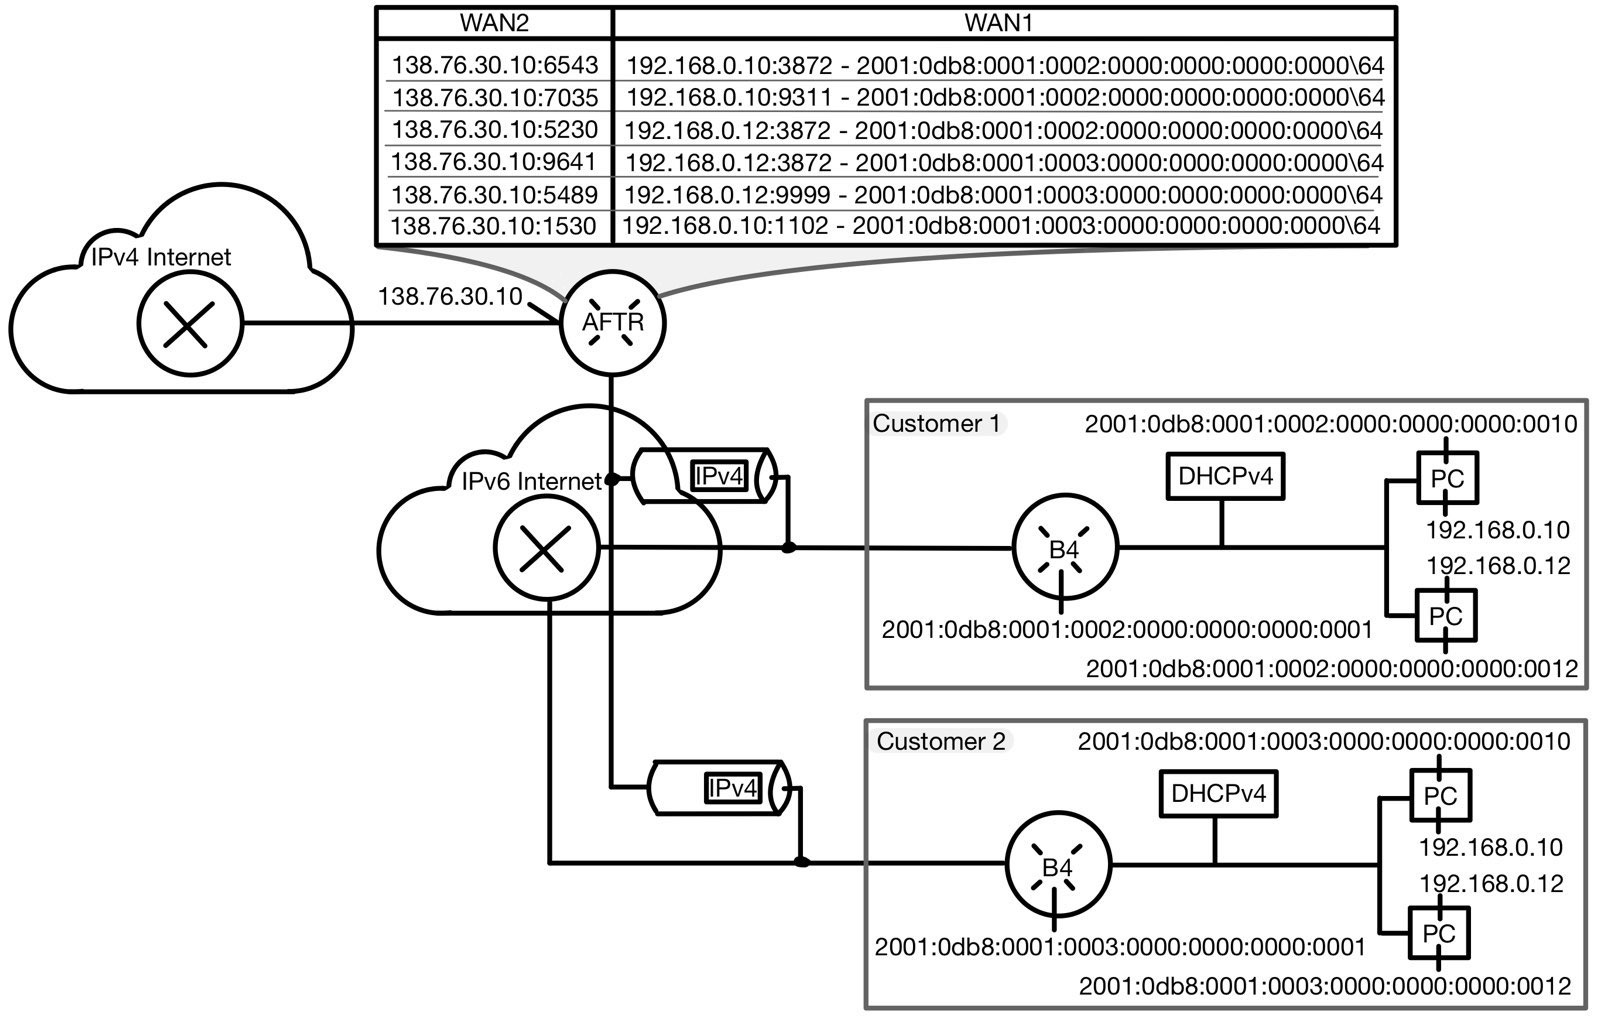
\includegraphics[width=0.5\textwidth]{images/dualstack_lite_network.png}
        \caption{Example of a Dualstack Lite network}
        \label{fig:dualstack_lite_network}
    \end{figure}
    \subsection*{END-USER IMPACT}
    \textit{Dualstack} and \textit{dualstack lite} provide the first real solution to the IPv4 exhaustion problem. They use IPv6 addresses. IPv6 addresses enable the end-user for the first time to get public, globally routable IP addresses for all their devices. This has many advantages but some disadvantages too. These will be discussed now.\\\\The introduction of IPv6 partially solves the NAT44 and NAT444 problem. Protocolls like IPSec or peer-to-peer protocols function out of the box, without any server, protocol extention or additional setup. IPv6 does not provide any NAT functionality and will never need it.\\\\Because each device has a unique IPv6 address, all ports are available for that device. Modern and future port intensive applications work without a problem.\\\\IPv6 enables new mulicast and broadcast features. With \textit{dualstack}, customers can experience IPTV seamlessly over IPv6 and profitate from the new features. VoIP also works better with IPv6. \\\\IPv6 enables end-to-end connectivity. This opens up better gaming multiplayer performance. Gamer do not have to care about different NAT types anymore.\\\\With direct true end-to-end TLS communication, a trusted channel between to parties can be established whithout a server and with use of client TLS certificates. This opens up new innovation possibilities for messanger apps and much more.\\\\The introduction of IPv6 to end-users with \textit{dualstack} and \textit{dualstack lite} has some downsides too. The main problem is regarding privacy. This will be discussed later on in this paper. \textit{Dualstack} and \textit{dualstack lite} have a security problem that is not related with IPv6 directly. Most devices accept IPv4 and IPv6 traffic. This leads to many firewall rules. System administrators and especially end-users can make many mistakes setting up the system. This can lead to exposed clients which are reachable over the internet eventhough they should remain private.\\\\All in all, \textit{dualstack} and especially \textit{dualstack lite} are the first good solutions for the IPv4 exhaustion problem. Apart from a more complicated and complex setup, the end-user gets new features and capabilities to use the internet. \textit{Dualstack} is the first step in the direction to return the internet to an open and accessable global network where everyone can host servers and access content.
    \section{LATEST SOLUTION: IPv6 ONLY}
    \lipsum[21]
    \subsection{TRANSLATION: NAT64/DNS64}
    \lipsum[22-24]
    \subsection{TRANSLATION: 464XLAT}
    \lipsum[24-26]
    \subsection{TRANSLATION: NAT-PT}
    \lipsum[26-28]
    \subsection*{END-USER IMPACT}
    \lipsum[18-21]

    \section{ISP Tunnels}
    \lipsum[21]
    \subsection{6in4}
    \lipsum[22-24]
    \subsection{4in6}
    \lipsum[24-26]
    \subsection{6to4}
    \lipsum[26-28]
    \subsection*{6over4}
    \lipsum[18-21]
    \subsection{6rd}
    \lipsum[26-28]
    \subsection*{Teredo}
    \lipsum[18-21]
    \subsection*{END-USER IMPACT}
    \lipsum[18-22]

    \section{Summary}
    \lipsum[100-104]

    %%section REFERENCES
    \bibliographystyle{plain}
    \bibliography{references}


\end{document}
